\documentclass[titlepage, a4paper, openbib, 10pt]{article}

%#####################################
%Usepackages en installingen
\usepackage[top=1in, bottom=1in, left=1in, right=1in]{geometry}
\usepackage[pdftex]{graphicx}
\usepackage{fancyhdr}
\usepackage{paralist}
\usepackage{sectionbox}
\usepackage[dutch]{babel}
\usepackage{chngcntr}
\usepackage{cite}
\usepackage{url}
\usepackage{makeidx}
\usepackage{enumitem}
\usepackage{tocloft}
\usepackage{listliketab}
\usepackage[table]{xcolor}
\usepackage{tabularx}
\usepackage{epsfig}
\usepackage{pdflscape}
\usepackage{pdfpages}
\usepackage{float}
\usepackage{multirow}
\usepackage{rotating}
\usepackage[utf8]{inputenc}
\usepackage{listings}
\lstset{language=C,
basicstyle=\ttfamily\footnotesize,
frame=shadowbox,
mathescape=true,
showstringspaces=false,
showspaces=false,
breaklines=true}

%\usepackage{showframe} %tmp
%#####################################
%Nieuwe commando's
\newcommand{\HRule}{\rule{\linewidth}{1pt}}
\newcommand{\organisatie}{\uppercase{Hogeschool Rotterdam / CMI}}
\newcommand{\modulenaam}{Numerical approximation for physics simulations}
\newcommand{\modulecode}{\uppercase{TINWIS01-8}}
\newcommand{\stdPunten}{2 ects}
\renewcommand{\author}{Gerard van Kruining, Giuseppe Maggiore}

\definecolor{lichtGrijs}{RGB}{169,169,169}



%#####################################
%Index en styling
\setlength{\cftbeforesecskip}{10pt}
\setlength\parindent{0pt}
\makeindex
\graphicspath{{img}}
\counterwithin{figure}{subsection}
\pagestyle{fancy}
\setcounter{secnumdepth}{5}
\setcounter{tocdepth}{5}

%#####################################
%     Alles voor header/footer
\fancyhf[HL]{\nouppercase{\textit{\leftmark}}}
\setlength{\headheight}{36pt}
\lhead{\uppercase{\footnotesize Module guide}}
\chead{\footnotesize \organisatie}
\rhead{
\includegraphics[width=0.09\textwidth]{img/logo}}

\lfoot{\scriptsize \modulenaam}
\cfoot{\scriptsize \today}
\rfoot{\small \thepage}

\renewcommand{\headrulewidth}{0.4pt}
\renewcommand{\footrulewidth}{0.4pt}
%#####################################

\begin{document}

%#####################################
%Titlepage
\begin{titlepage}
\thispagestyle{fancy}
\ 
\vspace{5cm}

\begin{center}

	
	\Large \textbf \organisatie
	
	\vspace{1.5cm}
	
	\HRule \\[0.4cm]
	
	\Huge \textbf \modulenaam
	
	\vspace{1.7cm}
	
	\Large \textbf  \modulecode
	
	\vspace{0.4cm}
	
	\HRule \\[1.5cm]
\end{center}
\vfill

% Author and supervisor
\begin{tabular}{l l}
	ECTS:  & \stdPunten\\
	Module responsible: & \author\\
\end{tabular}

\end{titlepage}

%####### Contentpagina ########
%\renewcommand{\baselinestretch}{1.5}\normalsize
%\tableofcontents
%\newpage
%\listoffigures
%\newpage
%\listoftables
%\newpage

%########### Inhoud ###########

\shadowsectionbox
\section*{Module description}
\begin{tabularx}{\textwidth}{|>{\columncolor{lichtGrijs}} p{.26\textwidth}|X|}
	\hline
	\textbf{Module name:} & \modulenaam\\
	\hline
	\textbf{Module code: }& \modulecode\\
	\hline
	\textbf{Number of ECTS \newline and number of individual study hours:} & This module gives \stdPunten ECTS, which corresponds to 56 hours.
	\begin{itemize}
		\item 5 $\times$ 120 minutes frontal lecture
		\item 3 $\times$ 120 minutes practicum
		\item the rest is individual study
	\end{itemize} \\
	\hline
	\textbf{Examination:} & Practical assignments \\
	\hline
	\textbf{Course structure:} & Lectures and practicums \\
	\hline
	\textbf{Required knowledge:} & All programming course, linear algebra. \\
	\hline
	\textbf{Learning tools:}  &
		\begin{itemize}
			\item Book: Game Physics, author: David Eberly
			\item Book: Friendly F\# (Fun with game physics), authors: Giuseppe Maggiore, Marijn Tamis, Giulia Costantini
			\item Text editors: Emacs, Notepad++, Visual Studio, Xamarin Studio, etc.
		\end{itemize} \\
	\hline
	\textbf{Connects to \newline competencies :} &
	\begin{center}
		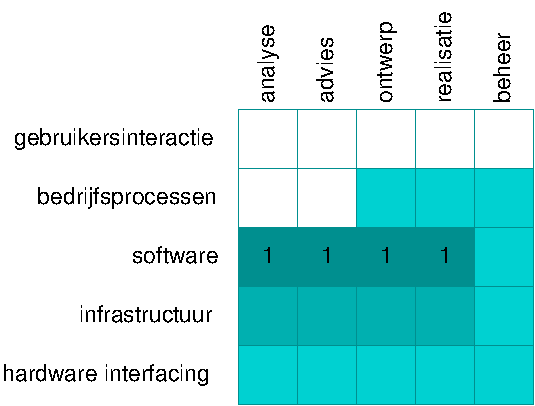
\includegraphics[width=7cm]{img/comptabel.pdf}
	\end{center}\\
	\hline
\end{tabularx}
\newpage

\begin{tabularx}{\textwidth}{|>{\columncolor{lichtGrijs}} p{.26\textwidth}|X|}
	\hline
	\textbf{Overall learning goal:}&
		The student is able to describe, define, and then implement numerical approximation techniques to physics simulations. \\
	\hline
	\textbf{Detailed learning goals:}&
	\begin{itemize}
		\item The student is able to distinguish the aspect of kinematics: linear and rotational motion, and associated forces (learning goal \textit{analysis});
		\item The student is able to give advice over the design and realisation of a kinematics simulation (learning goal \textit{advice});
		\item The student is able to design the structure and architecture of a kinematics simulation (learning goal \textit{design});
		\item The student is able to realise a working kinematics simulation (learning goal \textit{realisation});
		\item The student is able to communicate in correct Dutch or English, using the correct jargon, about physics simulations and kinematics, etc. (learning goal \textit{communication}).
	\end{itemize}
	\ \\
	\hline
	\textbf{Module responsible:} & \author\\
	\hline
	\textbf{Date:} & \today \\
	\hline
\end{tabularx}
\newpage

\newpage
\section{Algemene omschrijving}
	The overall goal of the course is to provide a detailed answer to the questions:	
	\begin{itemize}
	\item what are the kinematics equations?
	\item how does a physical simulation work?
	\end{itemize}
	
	In this section we discuss further the full breadth of what the course covers, plus the desired level of skills achieved by the students. 
	
	\subsection{Introduction}
		Simulation of the physical world is one of the most powerful fields of application of modern programming disciplines. Thanks to such simulations it is possible to set up virtual experiments, build virtual reality worlds, and many more modern complex applications. \\
		
		Since analytical solutions are very rarely available, building such simulations requires the use of approximation techniques, which themselves are also applied to many other fields such as computer vision, artificial intelligence, and robotics. \\

		The goal of the course is to provide a definition of the physical laws of kinematics, and of numerical approximations of complex dynamics. Moreover, we shall learn how to translate this knowledge into a working physical simulator. \\
				
	\subsection{Relationship with other teaching units}
		This module builds over all modules of programming, and is also strongly connected with previous knowledge about mathematics, and linear algebra. \\
	
	\subsection{Learning tools}
		Obligatory:
		\begin{itemize}
			\item Presentations and sources presented during lectures (found on N@tschool);
			\item Assignments to work on during practicums (found on N@tschool);
			\item Text editors: Emacs, Notepad++, Visual Studio, Xamarin Studio, etc.
		\end{itemize}
		Facultative:
		\begin{itemize}
			\item Book: Game Physics, author: David Eberly
			\item Book: Friendly F\# (Fun with game physics), authors: Giuseppe Maggiore, Marijn Tamis, Giulia Costantini
		\end{itemize}

\newpage
\section{Content}
	\paragraph*{Structure of lectures}
	The lectures are an adaptation of traditional frontal lectures. In order to improve attention and retention, the following interactive elements are also used:
	\begin{inparaenum}[\itshape i\upshape)]
	\item questions and quizzes to the class, followed by discussion;
	\item short group assignments, followed by discussion.
	\end{inparaenum}
	

	\paragraph*{List of topics}
	 	The following is a comprehensive and detailed list of the program of the course:
 		\begin{enumerate}
			\item Linear motion
			\item Rotational motion
			\item Linear acceleration
			\item Rotational acceleration
			\item Inertia tensor
			\item Euler integration
			\item Runge-Kutta integration
			\item Quaternions
			\item Time-derivative of matrices
			\item Time-derivative of quaternions
		\end{enumerate}
\ \\


\newpage
\section{Testing and evaluation}
	In this section we discuss the testing procedure of this course, and the grading criteria.
	
	\subsection{Overall description}
		
		This module is tested with a series of practical assignments. These assignments can be found on N@tschool. \\

		Foreword and notes:
		\begin{itemize}
			\item The practical assignments determine the final grade.
			\item The practical assignments are made up of elements of an interpreter or a compiler which is either incomplete or wrongly built. The students task is that of extending or fixing such elements.
			\item The practical assignments can be made in pairs.
			\item The practical assignments must contain extensive, individually written documentation.
		\end{itemize}
		\ \\
		
		This manner of examination is chosen for the following reasons:
		\begin{itemize}
			\item By reading existing sources students must read and reason about code (learning goals \textit{analysis} and \textit{advice}).
			\item By correcting or extending the sources students must write code (learning goals \textit{design} and \textit{realisation}).
			\item By writing documentation students must communicate about their code (learning goal \textit{communication}).
		\end{itemize}

		\ \\
		The grade of each practicum assignment is determined by:
		\begin{itemize}
			\item The correctness of the underlying physical and approximation rules (60\%).
			\item Completeness and clarity of the documentation (40\%).
		\end{itemize}

	\subsection{Assignments}
	
		\paragraph{Assignment 1 - linear motion}
			Students must define an Euler-integrated simulation over position, velocity (or linear momentum) and force.
			
		\paragraph{Assignment 2 - rotational motion}
			Students must define an Euler-integrated simulation over rotation, angular velocity (or angular momentum) and torque.
		
		\paragraph{Assignment 2B - Gram-Schmidt ortho-normalization}
			Students must define a Gram-Schmidt ortho-normalization.
			
		\paragraph{Assignment 2C - quaternions}
			Students must replace rotation matrices with quaternions.

		\paragraph{Assignment 3 - Runge-Kutta integration}
			Students must replace the Euler integration with a Runge-Kutta integration of order 4.

	\subsection{Grades}
		Assignments 1, 2, and 3 are obligatory. With these assignments the maximum grade possible is a seven. The other assignments are all optional and give each one and a half additional point.
		
\begin{tabularx}{\textwidth}{|>{\columncolor{lichtGrijs}} p{3cm}|X|}
	\hline
	\textbf{Assignments:} & \textbf{Value in grades} \\
	\hline
	1, 2, 3 & 7 \\
	\hline
	2B & 1.5 \\
	\hline
	2C & 1.5 \\
	\hline
\end{tabularx}
		

	\subsection{Deadlines}
		The assignments must be handed in, printed on paper, before the end of the last lecture on week 8 of the period. \textit{Herkansing} can be done by handing in the assignments before the end of week 1 of the following period (that would be right after the summer holiday).

	\subsection{Feedback}
		It is possible to discuss the assignments (and their evaluation) during the practicum lectures, or during week 10 of the period (the same holds for the \textit{herkansing}, but in reference to the following period).
		
%##############################

\newpage
%\bibliographystyle{plain}
%\bibliography{references}
%\newpage
\section*{Appendix 1: Examination matrix}
	\begin{tabular}{|p{7cm}|p{3.5cm}|p{5cm}|}
		\hline
		Learning goal & Dublin descriptors & Assignments \\
		\hline
		The student is able to distinguish the aspect of kinematics: linear and rotational motion, and associated forces
			& 1, 5
			& 1, 2 \\
		\hline
        The student is able to give advice over the design and realisation of a kinematics simulation
        	& 1, 3, 5 
        	& Documentation of all \\
		\hline
		The student is able to design the structure and architecture of a kinematics simulation 
			& 1, 3, 4
        	& 1, 2 \\
		\hline
		The student is able to realise a working kinematics simulation
			& 2 
			& All \\
		\hline
		The student is able to communicate in correct Dutch or English, using the correct jargon, about physics simulations and kinematics, etc.
			& 2 
			& Documentation of all  \\
		\hline
	\end{tabular}
	
	\vspace{1cm}

	Dublin-descriptoren:
	\begin{enumerate}
		\item Knowledge and insight
		\item Application of knowledge and insight
		\item Making judgments
		\item Communication
		\item Learning skills
	\end{enumerate}
	

%\newpage
%\section*{Bijlage 2: Voorbeeldtoets}

		Dit hoofdstuk bevat de beschrijving van de procedures om voor beoordeling in aanmerking te komen.\\
		Bijvoorbeeld voldoende aanwezigheid, 80\% van de opdrachten hebben ingeleverd, presentaties hebben verricht etc.\\

		Verder wordt zo gedetailleerd mogelijk beschreven hoe er tot een cijfer wordt gekomen en welke rollen er door docenten en ander betrokkenen hierbij vervuld worden. \\

		Geef een verantwoording van de toets; wat wordt getoetst, waarom is voor deze vorm gekozen.\\

		Vul een toetsmatrijs in voor de toets (zie bijlage).\\

		Beschrijf ook duidelijk de \textbf{herkansingsmogelijkheden}. \\

		Neem in geval van een schriftelijk tentamen een voorbeeldtoets op als bijlage.\\
		Geef daarbij per deelvraag het aantal te verdienen punten aan. \\

		Bij een schriftelijk rapport. Geef de beoordelingscriteria aan met daarbij de mogelijke score en de onderlinge weging. \\

		Toetsduur: \\

		Hoe en wanneer krijgt de student feedback?\\
%\newpage
%\section*{Bijlage 3: Studielast normering in ects}

		Dit hoofdstuk bevat de beschrijving van de procedures om voor beoordeling in aanmerking te komen.\\
		Bijvoorbeeld voldoende aanwezigheid, 80\% van de opdrachten hebben ingeleverd, presentaties hebben verricht etc.\\

		Verder wordt zo gedetailleerd mogelijk beschreven hoe er tot een cijfer wordt gekomen en welke rollen er door docenten en ander betrokkenen hierbij vervuld worden. \\

		Geef een verantwoording van de toets; wat wordt getoetst, waarom is voor deze vorm gekozen.\\

		Vul een toetsmatrijs in voor de toets (zie bijlage).\\

		Beschrijf ook duidelijk de \textbf{herkansingsmogelijkheden}. \\

		Neem in geval van een schriftelijk tentamen een voorbeeldtoets op als bijlage.\\
		Geef daarbij per deelvraag het aantal te verdienen punten aan. \\

		Bij een schriftelijk rapport. Geef de beoordelingscriteria aan met daarbij de mogelijke score en de onderlinge weging. \\

		Toetsduur: \\

		Hoe en wanneer krijgt de student feedback?\\
\printindex


\end{document}
